\textbf{Change this introduction to fit the final product!}
In this one year long project, we have collected results of a great number of materials with various structures and compositions. The initial experimentation was based on high-entropy silicides of the $Fe_2Si$ unit cell, created from the special quasi-random structure approach as described above. Despite the non-semiconducting character of this compound, we worked under the idea that the extraordinary properties that have been observed in high-entropy alloys through effects such as the cocktail effect, we could discover specific combinations of elements that would yield a semiconductor. In addition, the ratio between silicon atoms to metals allowed us to create nearly eqvimolar high-entropy alloys. 

Following this attempt, we transitioned into studying high-entropy silicides based on well known semiconducting 3d silicides such as $\beta-$\ch{FeSi2}, \ch{CrSi2} and \ch{MnSi_{1.75}}. The main outcome of this project is that for all 4 different starting silicides, we could only produce high-entropy silicides from one unit cell, furthermore in this cell only one specific compositions of elements was semiconducting. This was \ch{Cr_{0.25}Fe{0.25}Mn_{0.25}Ni_{0.25})Si2}, here-in CFMN, in the $\beta-$ \ch{FeSi2} crystal structure.  

This section will be structured in the following manner, firstly we will investigate the CFMN (fesi2) compound and various permutations of the composition. Thereafter we will look at other possible compositions of fesi2 based high-entropy silicides, and lastly test the CFMN composition in other crystal symmetries. In final we will present an overview of the complete study and the various compounds that have been investigated in order to propose promising directions and guideline future research directions in this field. In this way, we aim to understand the uniqe properties of CFMN (fesi2) and why this particular compound is semiconducting compared to the other testes structures in this project. Properties we will cover is the overall stability by total energy and corresponding enthalpy of formation, the magnetic properties and which elements contribute to the magnetism. But in majority, we will look at the band gap and related properties, as this is the main motivation and distinction of the study.    

\chapter{The results of \ch{(CrFeMnNi)Si2} in the $\beta-$\ch{FeSi2} structure}
\label{sec:good}

$\beta-FeSi_2$ in the orthorombic cmce crystal lattice is a well known semiconductor with an experimentally measured band gap of around 0.8 ev \textbf{cite}, the nature of the band gap is under debate, all though most ab inito studies point to an indirect gap, experimental work indicate a direct gap. From our own DFT calculations, we find an indirect band gap close to 0.65 eV with PBE. This is in good agreement with other meassurements from ab intitio studies \textbf{cite materials projects, other studies.} 

The density of states and charge density of bulk $\beta-$\ch{FeSi2} from PBE calculations can be seen in figure .., ..  From the figures we observe a clear band gap and semiconducting character. Moreover, we note from the density of states that the gap is identical in both spin channels, indicating that this material is diamagnetic. We find this to be true from the written magnetization in VASP, this also is in agreement with relevant literature \textbf{cite}. \textbf{Find reference for $\Delta H^0$.} Finally, the enthalpy of formation of this compound is -18.6583 eV.

\section{Eqvimolar SQSs}

\subsection{Introduction}

The CFMN alloys of the fesi2 unit cell alloys can be seen in figure ... The supercells consist of 48 atoms, 16 of which is evenly distributed between Cr, Fe, Mn, and Ni, the remaining 32 sites occupied by silicon atoms. Bellow in table .. we list the total energy per atom (Toten), final magnetic moment per atom (Mag), and the band gap of the five distinct SQSs corresponding to the CFMN (fesi2) compound. In addition we include the mean and standard deviation of the values, plus the enthalpy of formation. For simplicity, we denote the SQSs as A, B, C, D and E.

\begin{table}[H]
\centering
\begin{tabular}{@{}cccc@{}}
\toprule
Structure  & Toten (eV) & Mag (?) & Band gap (eV) \\ \midrule
\textbf{A} & −6,6080                & 0.0833                    & 0.0280        \\
\textbf{B} & −6,6138                & 0.0833                    & 0.0523        \\
\textbf{C} & −6,6063                & 0.0834                    & 0.0344        \\
\textbf{D} & −6,6155                & 0.0833                    & 0             \\
\textbf{E} & −6,6089                & 0.0833                    & 0.0495        \\ \midrule
\textbf{Mean} & -6.6105 & 4.0000 & 0.0328    \\
\textbf{Std} & 0.0039 &  0.0000 &  0.0210 \\
\textbf{$\Delta H_{mean}^0$} & -11.5000 eV & - & - \\ \bottomrule
\end{tabular}
\caption{Total energy per atom, final magnetic moment, band gap (GGA) and formation enthalpy of $Cr_4Fe_4Mn_4Ni_4Si_{32}$ SQSs based on $FeSi_2$}
\label{table:fesi2_summary}
\end{table}  

\textbf{Write a section on magnetism in method}
From a first glance, we observe very similar properties between the SQSs regarding both the total energy and final magnetic moment. Comparing to bulk \ch{FeSi_2}, this compound is both less stable, from the enthalpy of formation, and magnetic. For the magnetic character of the compound, we performed self-consistent total energy calculations with three diffrent magnetic configurations, non-magnetic (ispin=1), colinear magnetism with the initial magnetic moment equal to 1 times the number of ions, and lastly two times N ions. Of the three starting positions, we found the two latter to yield near identical total energies, with the middle seting winning out in some SQSs. The consistent magnetic moment between the 5 supercells is excpected seeing as all 5 structures consist of equivalent elements. The magnetic moment observed is solely attributed from 3d electrons and in particular those of chromium and manganese atoms. 
 
\subsection{The band gap} 
 
The most interesting property of these SQSs is in fact the band gap. We note a mean band gap of about 0.03 eV, much lower than 0.65 eV of bulk $FeSi_2$. But a band gap in this smaller range makes for  excellent application in for instance thermoelectrics. The gap is seen in 4 out of 5 SQSs, but surprisingly not in the most stable arrangement (D), the largest gap observed is about 0.05 eV from structure B, which is slighlty bellow D in terms of total energy, but still a way above the mean energy. Similar to the bulk material, also these band gaps are indirect, the transitions are listed bellow in table .. .     

\begin{table}[H]
\centering
\begin{tabular}{@{}ccc@{}}
\toprule
Structure  & Gap (D/I) & Transition                              \\ \midrule
\textbf{A} & I         & (0.500,0.333,0.500) $\rightarrow$ (0.500,0.000,0.000)  \\
\textbf{B} & I         & (0.250,0.000,0.250) $\rightarrow$ (0.000,0.000,0.000)  \\
\textbf{C} & -         & (0.500,0.000,0.500) $\rightarrow$ (-0.250,0.333,0.500) \\
\textbf{D} & I         & -                                        \\
\textbf{E} & I         & (0.000,0.000,0.000) $\rightarrow$ (0.250,0.000,0.250)  \\ \bottomrule
\end{tabular}
\caption{Band gap transition of CFMN (fesi2) SQSs with PBE functional}
\end{table}

A very useful method to extract information regarding the band gap of a material is to plot and study the band structure, however this is not as insightful when considering large supercells consisting of several elements and a  large number of energy bands. The solution to this is normally to do a band unfolding, but given the complex structure and implementation of SQSs in VASP proved difficult. Instead we investigate the band gap from the plotted density of states shwon in figure 8.1. We only include the DOS of this particular super-cell because results of the most stable arrangement is probably the most representative of a potential high-entropy silicide, nevertheless we will consider the remaining SQSs in the following sections as well.  

\begin{figure}[H]
	\centering
	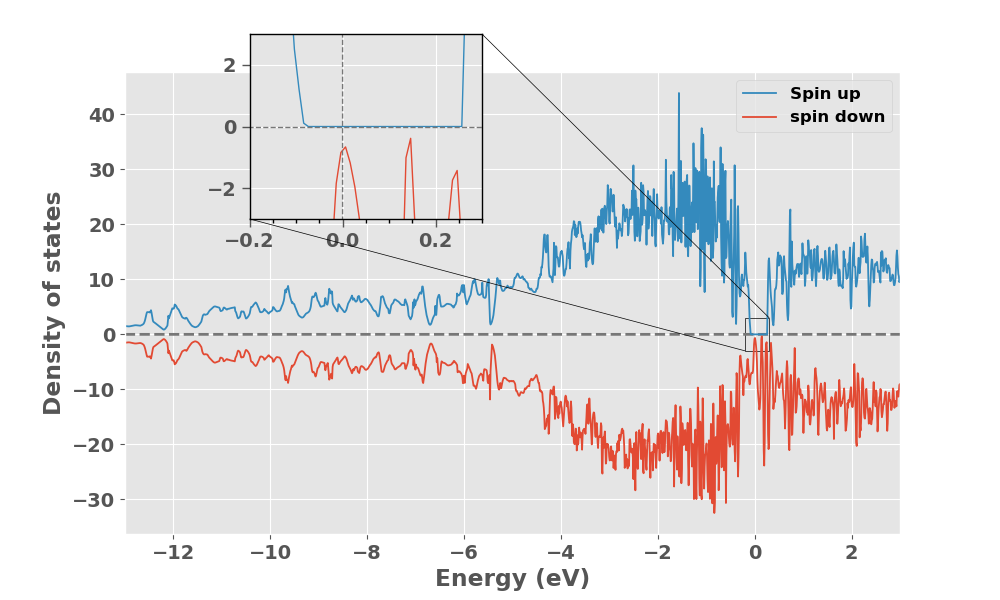
\includegraphics[width=\textwidth]{results/fesi2/D_TDOS.png}
	\caption{Density of states SQS D CFMN (fesi2) from PBE calculation}
\end{figure}

From the DOS we observe that the band gap in this structure differ between the spin up states and spin down states, following the magnetic property of the material seen in table 8.1. In this particular SQS the spin down channel is completely metallic, and the spin up channel exhibit a relatively large band gap, thus we can classify this SQS as either a half-metal, or possibly a spin-gapless conductor (\textbf{Insert references/discuss this}). Furthermore we find that the band gap in all SQSs of this alloy is severely spin-polarized in the spin up direction \textbf{Is this okay to say?}. We list the spin-dependent band gaps in table 8.3, and show the relationship in SQS B in figure 8.2 bellow.

\begin{figure}[H]
	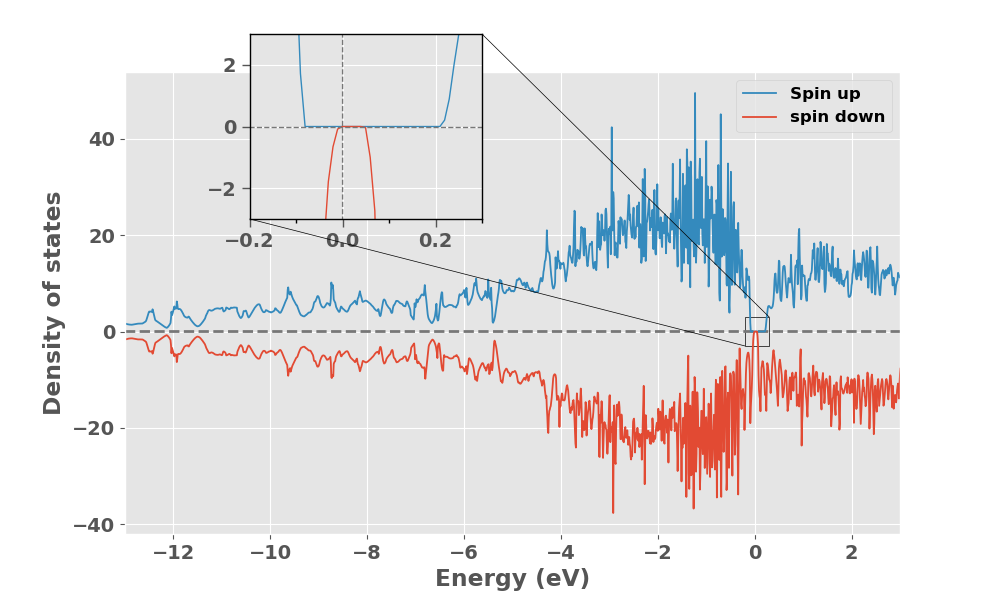
\includegraphics[width=\textwidth]{results/fesi2/B_TDOS.png}
	\caption{Density of states SQS B CFMN (fesi2) from PBE calculation}
\end{figure}

\begin{table}[H]
\centering
\begin{tabular}{@{}cccc@{}}
\toprule
Structure  & Spin-up & Spin-down & Total  \\ \midrule
\textbf{A} & 0.0814  & 0.0522    & 0.0281 \\
\textbf{B} & 0.2932  & 0.0523    & 0.0523 \\
\textbf{C} & 0.2355  & 0.0343    & 0.0343 \\
\textbf{D} & 0.3386  & 0         & 0      \\
\textbf{E} & 0.3078  & 0.0495    & 0.0495 \\ \bottomrule
\end{tabular}
\caption{Band gap (eV) with PBE in spin up and spin down channels of CFMN (fesi2) SQSs}
\end{table}

From table 8.3 we find that SQSs B, D and E all display band gaps around 0.3 eV in spin up, and small non-zero or zero band gap in the case of SQS D in spin down. In the coming section we will investigate the band gap and electronic structure of this compound by looking at the local and projected density of states. 

\subsection{Local and Projected density of states}
From LDOS and PDOS it's possible to study the above case by the contributions of the individual elements in the structure. In the local density of states plotted in figures 8.3 and 8.4 we see that the s-electrons in Si occupy states in the lower energy regions and the p electrons at energies closer to the Fermi energy, while both equally occupy states above $E_F$. In the transition metals we see that 3d electrons dominate across the energy range. Between the different TMs we observe that 3d electrons particularly of manganese and chromium show a strong presence in spin down right above $E_F$, and just bellow in the spin up direction. Meanwhile iron and nickel lie at lower energies respectively. The relationship and interaction between the different elements can better be seen in the projected density of states in figure 8.5. 

\begin{figure}[H]
	\centering
	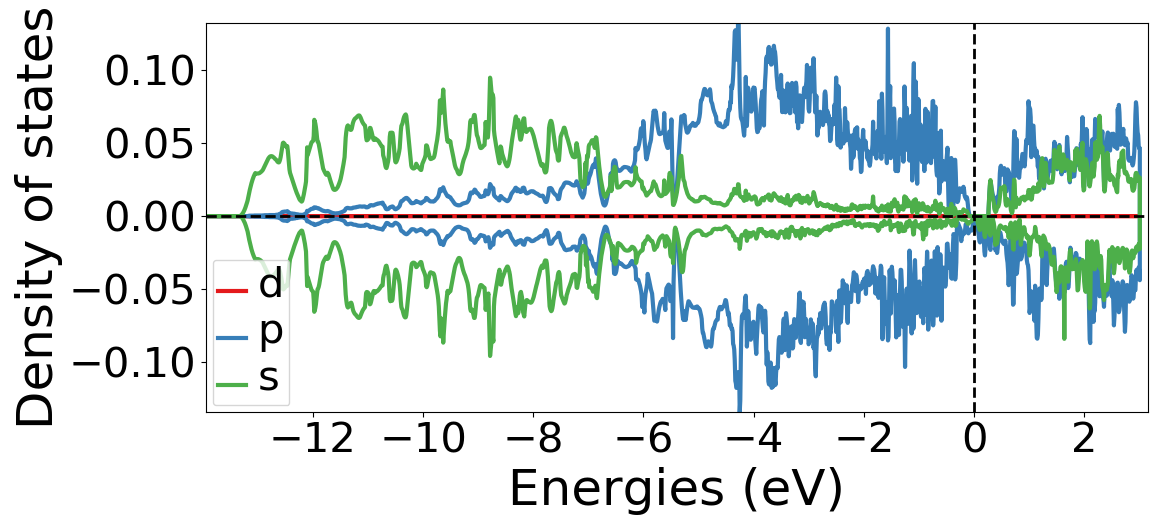
\includegraphics[width=.7\textwidth]{results/fesi2/D_LDOS_Si.png}
	\caption{Local density of states of Si (SQS D)}
\end{figure} 

\begin{figure}[H]
	\centering
	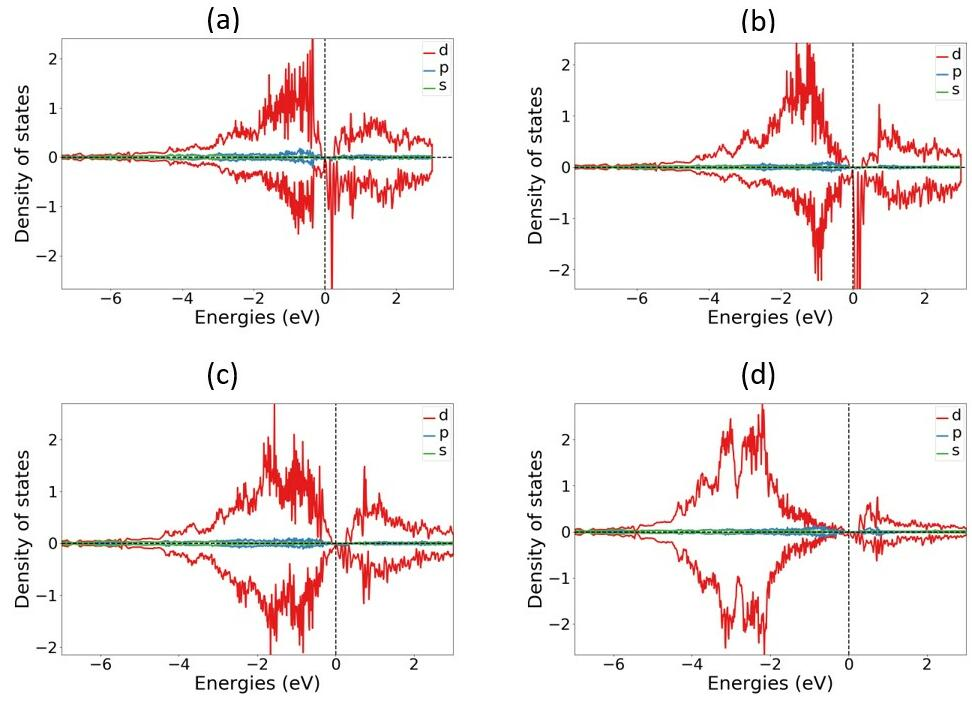
\includegraphics[width=\textwidth]{results/fesi2/D_LDOS.jpeg}
	\caption{Local density of states of TMs (SQS D), (a) Cr, (b) Mn, (c) Fe, (d) Ni}
\end{figure} 

\begin{figure}[H]
	\centering
	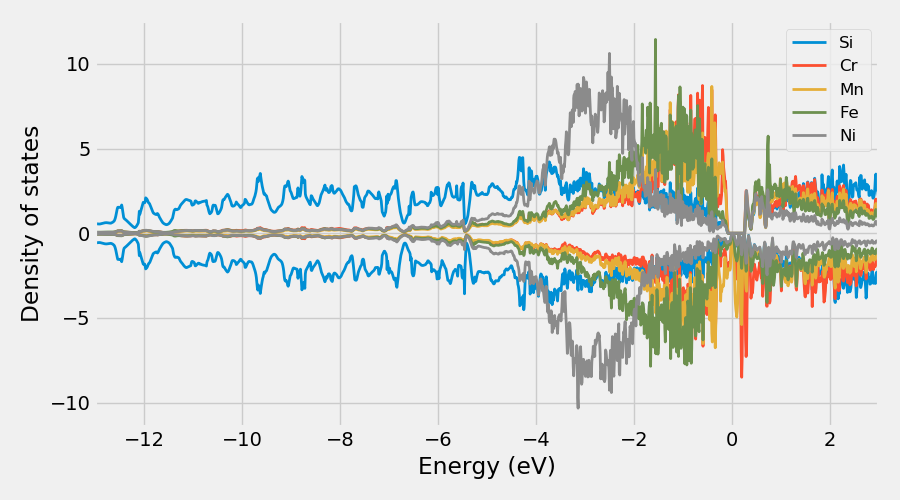
\includegraphics[width=.8\textwidth]{results/fesi2/D_PDOS.png}
	\caption{Projected density of states SQS D CFMN (fesi2) from PBE calculation}
\end{figure} 

In agreement with the local DOS we observe here that the Si s-electrons occupy the lower energetic states, and evidence of p-3d hybridization at higher energies. With the upmost energetic states in the valence band occupied by 3d electrons of chromium and manganese. Bellow we include the PDOS of SQS D and B but focused around $E_F$, from these figures we find that the spin down channel in D contain a more dominant presence of manganese especially, and some chromium as compared to the semiconducting SQS B.  
  
\begin{figure}[H]
	\centering
	\begin{subfigure}{.45\textwidth}
			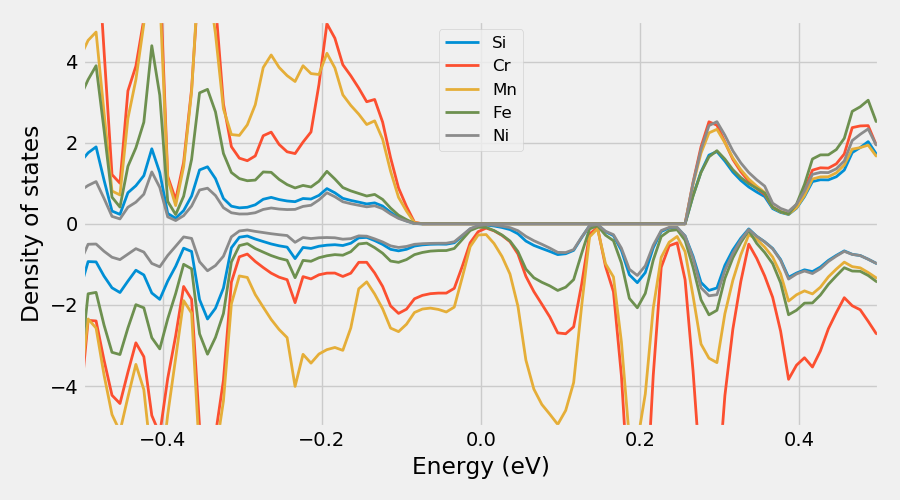
\includegraphics[width=\textwidth]{results/fesi2/D_PDOS_Ef.png}
			\caption{SQS D}		
	\end{subfigure}
	\hspace{0.5cm}
	\begin{subfigure}{.45\textwidth}
		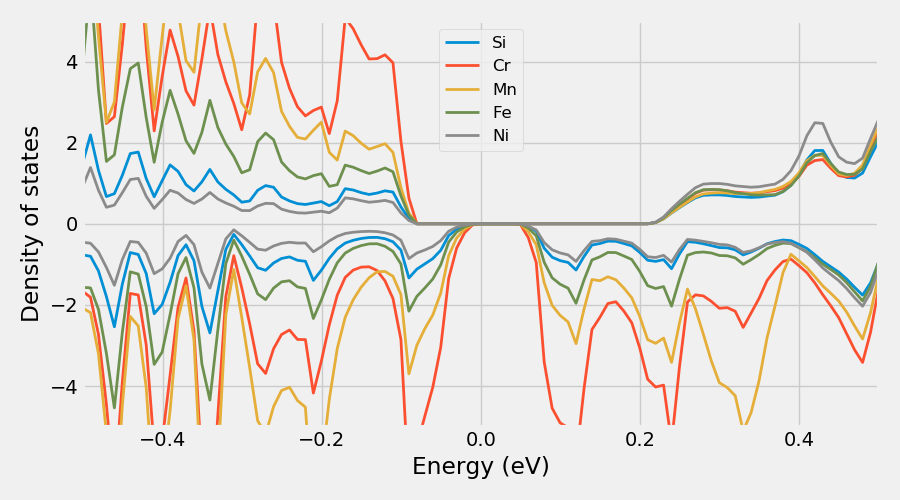
\includegraphics[width=\textwidth]{results/fesi2/B_PDOS_Ef.png}
		\caption{SQS B}		
	\end{subfigure}
	\caption{Projected density of states of SQS D and B around $E_F$}
\end{figure}

In the context of DFT and VASP there are several factors than can affect the accuracy of the DOS. As mentioned in section .., the type of numerical smearing is paramount for accurate DOS calculations. In this project we experienced large differences between calculations from gaussian and TBC smearing in relation to the band gap and DOS, this will be covered in more detail later. Moreover the DOS is very sensitive to computational factors such as the number of points (NEDOS in VASP) and the number of k-points (to solve the DOS integral, see section ..). For example, the band gap in structure C could only be seen in the density of states when increasing the number of points in the DOS from 2401 to 20000 points. This is shown bellow in figure .., where we plot the density of states around the fermi energy, denoted by the stippled red and blue lines, relative to the density of states with 2401 points and 20000 points respectively, all other parameters remained unchanged. It should however be noted that the second calculations applied the charge density calculated by the former for quicker convergence. 

\begin{figure}[H]
	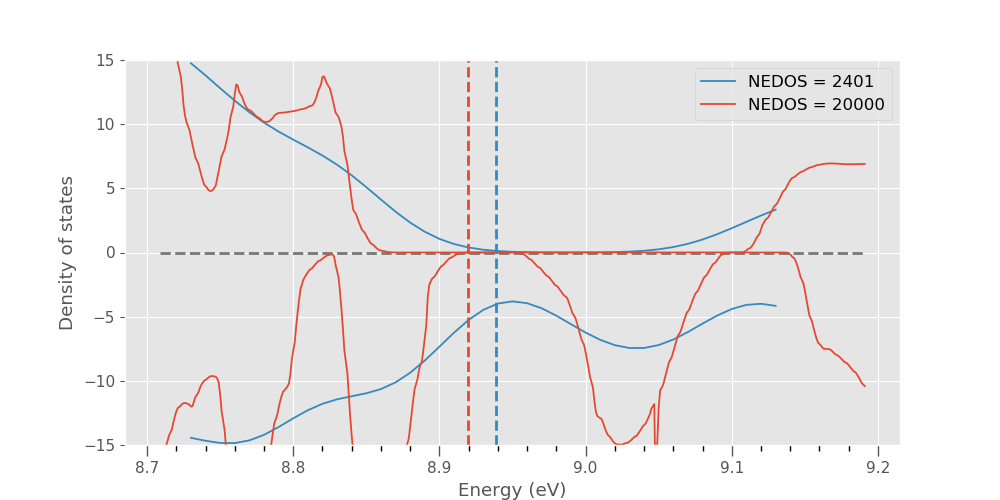
\includegraphics[width=\textwidth]{results/fesi2/C_DOS.png}
	\caption{Density of states of SQS C with 2501 points vs 20000 points in the density of states.}
\end{figure} 

Despite of the higher accuracy of the greater number of points, we continue to perform calculations with around 2400 points, mostly down to the increased workload of analyzing the DOS with such a large number of points. 
 
\textbf{Some way of visualizing the eigenvalues?}
To explain the result of SQS D in comparison to the other semiconducting SQSs of the alloy, we look at the calculated eigenvalues for the distinct supercell. Here it's seen that eigenstates transition between full to empty occupancy at energy band 124 in spin down and 129 in spin up, thus a difference of 5 bands between states in the different spins, this is also the case in the other SQSs. In particular of SQS D however is that for a majority of k-points the bands 124 and 125 contain occupancy values other than 1 and 0 for the spin down states. These are either non-physical values above 1 or negative, in other words indicating states are more than filled or less than empty. Or values in-between 1 and 0, meaning partially filled states (defect states). If we were to neglect these defect states and only consider bands where the occupancy is above 0.99 or bellow 0.01, the band gap of structure D remain consistent in spin up, but we now observe a band gap of around 0.05 eV in the spin down channel as well. Again, this would have been extremely insightful to investigate with the help of a band structure diagram. The non-physical values is simply a consequence of using the tetrahedron method with Bloch corrections (ISMEAR-5) as numerical smearing, (\textbf{Insert reference}). Interestingly we only find such values for spin channels also containing defect states. Furthermore the presence of such defect/non-physical states is found as the key divider between structures with and without a band gap also for the coming examples in this project. 

\subsection{Meta-GGA and hybrid functional}

As expressed previously, in this work we invoke 3 level of depths GGA (PBE), meta-GGA (SCAN) and hybrid functionals (HSE06) to determine the band gap of the SQSs. In table .. bellow we list the respective band gaps of these methods for all 5 SQSs of CFMN (fesi2). Note that all calculations is done with TBC smearing.

\begin{table}[H]
\centering
\begin{tabular}{@{}cccc@{}}
\toprule
Structure  & PBE    & SCAN   & HSE06  \\ \midrule
\textbf{A} & 0.0281 & 0.0000 & 0.0207 \\
\textbf{B} & 0.0523 & 0.0890 & 0.1808 \\
\textbf{C} & 0.0344 & 0.0690 & 0.0196 \\
\textbf{D} & 0.0000 & 0.0000 & 0.0000 \\
\textbf{E} & 0.0495 & 0.1048 & 0.0133 \\ \bottomrule
\end{tabular}
\caption{Band gap of CFMN (\ch{FeSi2}) SQSs with GGA (PBE), meta-GGA (SCAN) and hybrid-functionals (HSE06).}
\end{table}

The most obvious result of table .. is that aside from SQS A, all 3 methods agree on the presence of the band gap. This in itself is a very positive result for this project, as the primary motivation is based simply on locating semiconducting high-entropy silicides and thus the agreement of 3 different methods on the same structures is most welcome. On the other hand, it's clear that the actual size of the gap is under some debate. We note the largest observed band gaps is largely associated with the SCAN functional, compared to PBE calculations this result is very in line with what is expected by involving more complex factors in the calculations, as discussed in section .. In contrast, by the same argument we would not expect that par SQS B, the overall smallest band gaps is found with the well-proven hybrid functional HSE06, as shown in table .. The results associated with the HSE06 functional will be covered in more detail in the subsequent section, for now lets consider SCAN. 
 
\paragraph{SCAN \\}
On the surface the results with SCAN are sensible and in line with the PBE results with the exception of SQS A, in this case the calculations with SCAN resulted in a zero band gap as opposed to 0.03 eV with the PBE functional. However also the SCAN results of the other 4 SQSs differ from the PBE band gaps. In the two SQSs B and E the band gap is increased with SCAN, but the properties of the gap is reversed compared to PBE. This is shown in figure 8.8 for SQS E. The band gap of this SQS as previously described is around 0.3 eV in spin up and 0.05 eV in spin down equaling a total 0.05 eV band gap. Bellow in figure 8.8 it's seen that the SCAN functional results in a larger total gap of 0.09 eV, but at the same time lowers the previously large spin up gap, and increase the smaller spin down gap. This is also seen in SQS B. In structures C and D this is taken a step further and reverse the spin polarization of the band gap. \textbf{Include figure?}. For example, in despite of the SCAN functionals agreement with PBE of predicting a zero total band gap in SQS D, the former in opposite of PBE find a band gap in the spin down channel.  
 
\begin{figure}[H]
	\begin{subfigure}{.5\textwidth}
		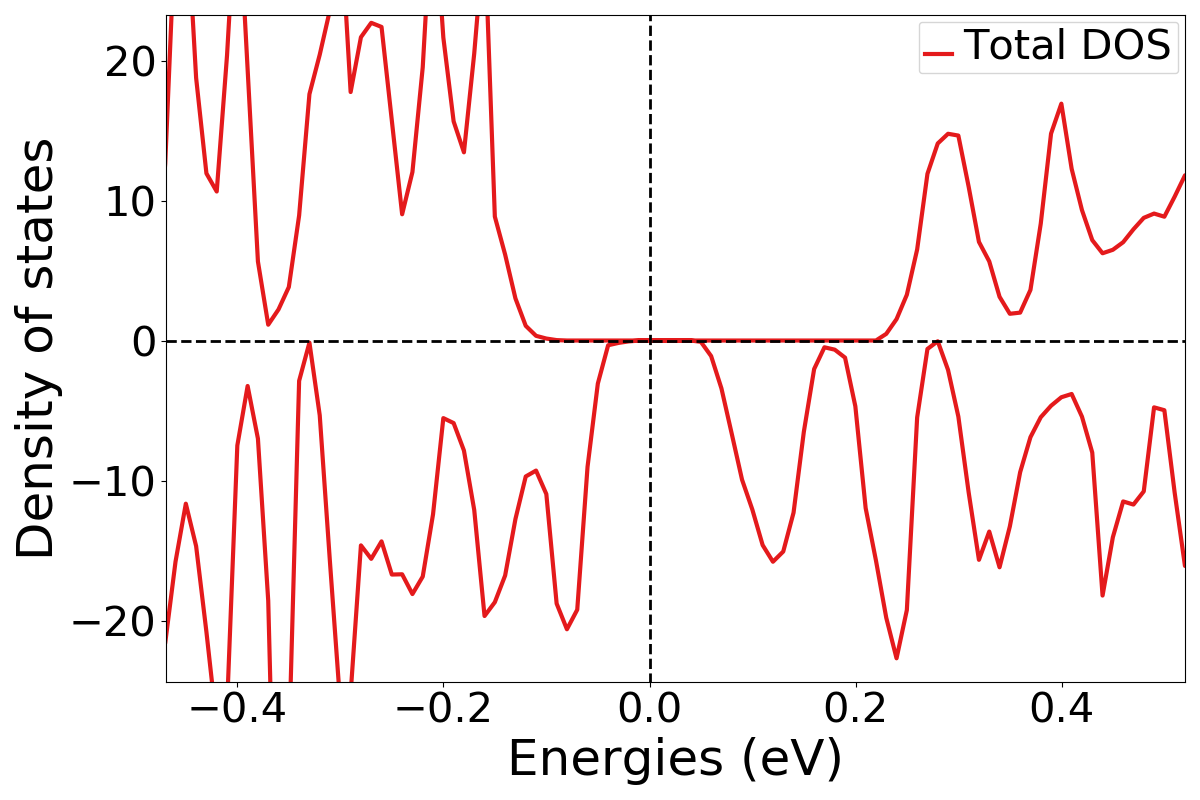
\includegraphics[width=\textwidth]{results/fesi2/E_DOS_pbe.png}
		\caption{PBE}
	\end{subfigure}
	\begin{subfigure}{.5\textwidth}
		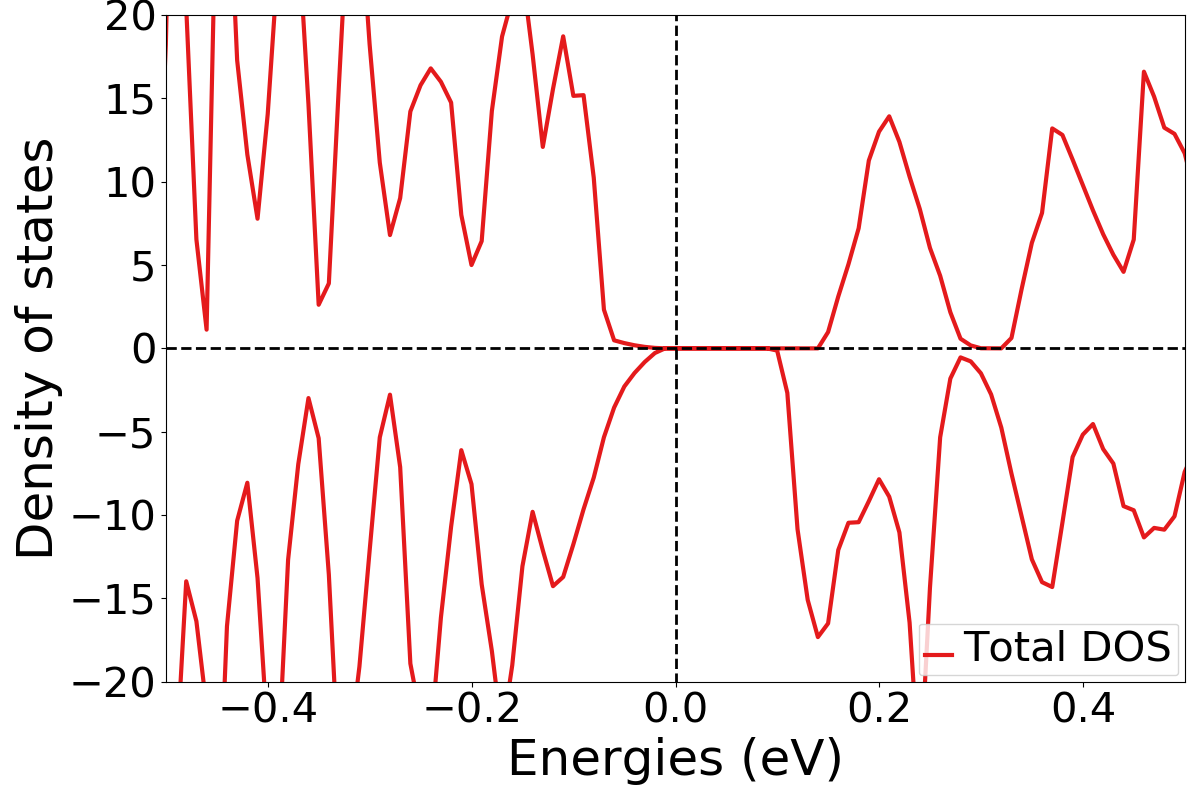
\includegraphics[width=\textwidth]{results/fesi2/E_DOS_scan.png}
		\caption{SCAN}
	\end{subfigure}
	\caption{Density of states of SQS E illustrating the different band gap from calculations with (a) PBE and (b) SCAN functional}
\end{figure}

\paragraph{HSE06 \\}
As stated above, the measured band gaps with the HSE06 functional was less than that of PBE and SCAN for most of the tested SQSs. Hybrid functionals as described in section .. is computationally demanding, but comes with superior accuracy for band gap measurements, and the HSE06 functional in particular is on the top of the list. For this reason, one would in general expect larger band gaps compared to GGA or meta-GGA calculations, as highlighted in .. \textbf{cite?} The one exception we observed to this trend is in SQS B (figure 8.9 A), here the band gap increase from 0.05 eV to 0.09 eV and 0.18 eV from PBE to SCAN to HSE06. One possible reason behind the abnormally large gap can originate from the small number of k-points we had to employ in order for the calculations to converge. Recalling that the gap transition in in the PBE calculation was (0.250,0.000,0.250)-(0.000,0.000,0.000), compared to the hybrid functional we now see that the transition is between k-points (0.500,0.000,0.000) and (0.000,0.000,0.000). Moreover, the point (0.250, 0.000, 0.250) in k-space is not included in the hybrid functional due to the narrow mesh (this we read from the IBZKIT file in VASP). Thus it's a possibility that the large gap is caused by the fact that the minimal gap is not encapsulated by the k-points in the HSE06 calculation. However we also see this trend in the other SQSs, but despite of the different transistion in k-space, these structures find lesser band gaps with the HSE06 functional compared to PBE. Additionally, we find similar results in the bulk $\beta-$\ch{FeSi2} structure. In this calculation we applied the same number of k-points for HSE06 as for PBE and SCAN. Nevertheless we find a much larger band gap of around 1.5 eV with HSE06, as opposed to 0.65 eV with both PBE and SCAN, and as mentioned before the two latter is in much better agreement with experimental results and ab intio work on the band gap of $\beta-$\ch{FeSi2} \textbf{cite materials project, other articles}. Additionally also in this case, the transition vary between functionals. PBE: (0.000,0.000,0.000)-(0.000,0.000,0.250), and HSE06: (0.000,0.000,0.000)-(0.000,0.000,0.500). \textbf{Include band-diagram for bulk fesi2?} 

\begin{figure}[H]
	\centering	
	\begin{subfigure}{.8\textwidth}
		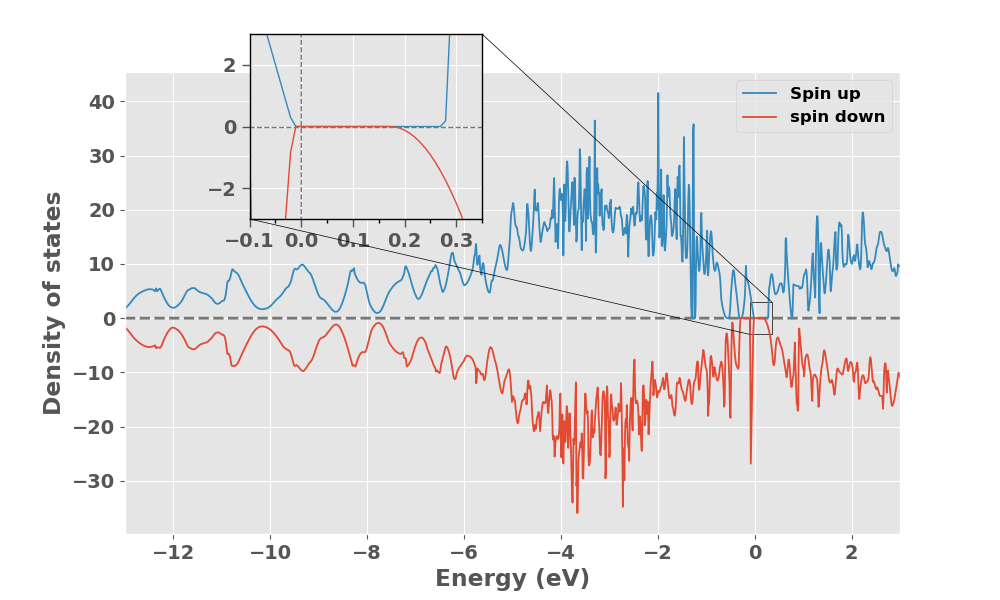
\includegraphics[width=\textwidth]{results/fesi2/B_TDOS_hse06.png}
		\caption{SQS B}
	\end{subfigure}
	\begin{subfigure}{.8\textwidth}
		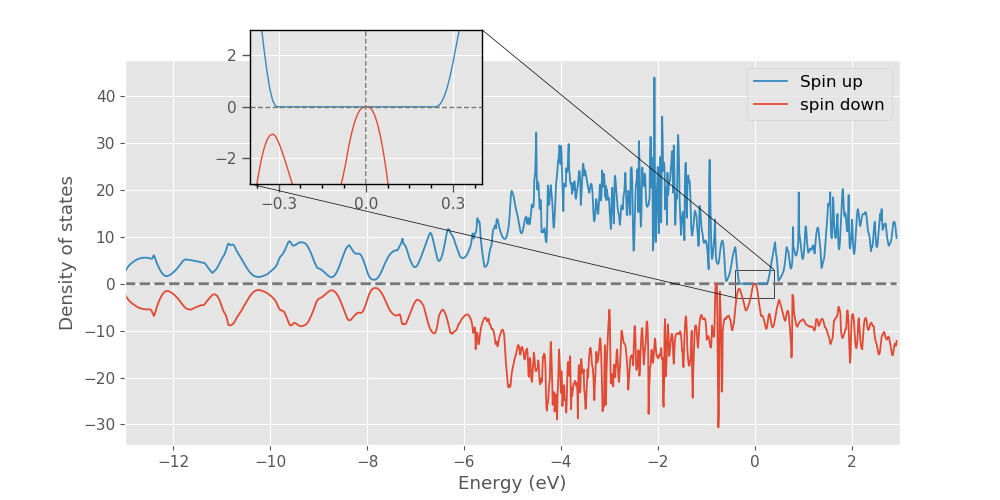
\includegraphics[width=\textwidth]{results/fesi2/E_TDOS_hse06.png}
		\caption{SQS E}
	\end{subfigure}
	\caption{Total density of states of SQS (a) B and  (b) E from calculations with HSE06}
\end{figure}

Aside SQS B, we generally see good agreement between HSE06 and PBE calculations. In A we notice that the 0.02 eV band gap stems from a 0.7 eV gap in spin up and 0.02 eV in down. Likewise SQSs C, D, and E all exhibit large band gaps in spin up, 0.17, 0.37 and 0.55 eV respectively, and correspondingly very narrow spin down gaps 0.032, 0, and 0.013 eV. In figure 8.9 above we include the plotted density of states for SQS B (a) and E (b) clearly illustrating the spin polarization in E. Compared to the listed spin dependent band gaps from PBE in table 8.3, we see that the band gaps from HSE06 typically compares or exceeds in spin up, and lessen in spin down, with the exception of SQS B (0.29 eV and 0.18 eV) where also the spin down gap is increased. 


\paragraph{Numerical smearing \\}
\textbf{Rewrite/reconsider this paragraph, is it needed? How can I write this more concise? Figure?}
One final point we would like to cover in the discussion of HSE06 calculations of this system, and generally in this project, is the effect of smearing on the reported band gaps. From the method section, we know that TBC smearing is the preferred choice for accurate density of states and total energy calculations of semiconductors, alike we know that this method is unfitting to calculate the forces in metals. As discussed in the methodology section, hybrid functionals proved difficult to converge for such composistionally complex structures, thus we were forced to initially calculate the charge density from the HSE06 functional with did a self-consistent calculation with gaussian smearing and smearing width of 0.05 eV. Thereafter reuse the calculated charge density for subsequent hybrid calculations with TBC smearing. Using SQS A as an example, from the first run (Gaussian), the band gap is 0.15 eV, (0.78 up and 0.15 down). However the eigenvalues contain defect states and the band gap is not observable from the density of states. Next we can reapply the charge density to perform an additional HSE06 calculation with gaussian smearing, but reducing the smearing width from 0.05 eV to 0.005 eV. Now we find a new gap of 0.1 eV (0.21 up and 0.1 down), with no defects in the eigenstates, and apperant in the density of states. In cases where we find conflicting results between the eigenvalues and density of states we rely on the script bandgap.py provided in the pymatgen package, refer to section .. for a description. With this we only report a band gap for the HSE06 calculation with TBC smearing, note that this method return the same value of the gap as well. As another example lets consider SQS B. In contrast, the nummerical smearing does not appear to impact the band gap of this structure. We find from HSE06 simulations with gaussian smearing of both 0.05 and 0.005 eV smearing width to yield results around 0.28 eV and 0.18 eV in spin up and down. But alike SQS A, the larger smearing width comes with a few defect states in the spin down channel and additionally can not be seen in the density of states. However, particular of this structure is that the bandgap.py script validate the calculated total band gap from the eigenvalues in all three calculations. Aside from this abnormalty, the other SQS similar to A find some similarities between smearings, but only TBC was validated with bandgap.py, furthermore the DOS does not with the same clarity reproduce the calculated band gap from the eigenvalues in calculations done with gaussian smearing compared to TBC. \textbf{figureof the DOS of hybrid/smear/smear5 maybe A?}

We see from the above examples that as most studies and articles state, that TBC smearing is superior in terms of accurate total energy and DOS calculations of semiconductors. Similar to how TBC produce inacurate forces of metals, in several cases in this project we relaxed the structures with gaussian to forces bellow 1E-2, but subsequent calculation with TBC in certain cases resulted in forces above 0.1, without making any geometric alteration to the previously relaxed cell \textbf{(Include examples?)}. On the grounds of these factors we can report good agreement between our own results and the theoretical advice regarding numerical smearing in DFT studies \textbf{Insert refrences}

\textbf{Figure on cpu time pbe vs scan vs hse06.}

Fro the above examples between it's clear that the band gap in this compound is subject to the SQS and the applied exchange-correlation functional. From the SCAN functional we found several cases that disagreeed with the PBE results, see SQS A, C and D. Combining this with the popularity and wide-spread application and reliability of the PBE functional. See for example materials project, that exclusivly list PBE band gaps, and other relevant studies \textbf{refrences}. We put the most faith in the PBE results. An additional point is that GGA is known to underestimate band gaps, due to the concepts described in section .., therefore if we find a gap with PBE, the real material would most probably also have a band gap, and a larger one at that.

Regarding the HSE06 functional, the inaccuracy shown for the bulk material is concering, escpecially considering the lack of experimental baselines in this study to compare and measure our results after. However, generally we find much better cohesion between PBE and HSE06 compared to SCAN for the 5 supercells, both methods predict semiconductors with heavy spin polarization in the spin up direction, par B. The fact that all 3 functionals and five structures for the most part agree on the presence of a semiconductor is a overwhelmingly positive result in itself, that allow us to state with high certainity that this compound is in fact a semiconductor, or we may label the compound as a half-metal or spin-gapless conductor from the registered spin dependence. A qualitative study on the exact band gap would demand a much greater scope as there are many factors affecting the value that we have neglected. One of these is the randomness involved with SQSs. For instance, by increasing the SQS size, ie number of atoms in the supercell, we found again different band gaps, but still, the presence and characther of the compound was consistent. \textbf{Include this? Table?} To draw any meaningfull conclusions on the size of the band gap would requiere us to both increase the number of SQS's of the composistion due to the obseved variation in the band gap between the 5 tested supercells, and as well for different supercell sizes to obtain some sort of convergence of the band gap. On the other hand, if we were to go by the most stable configuration of this narrow study, then this alloy would be labeled as a half-metal from the results of SQS D across all three functionals.  

\subsection{Probability distribution functions and charge density}

In this final segment of the CFMN alloys we will look at the probability distribution functions and charge density. We only include the results of SQS B and D as an in-depth across 5 unieq structures become tedious and time-consuming, the PDFs of the remaining structures can be seen in appendix .. 
 
\begin{figure}[H]
	\centering
	\begin{subfigure}{\textwidth}
		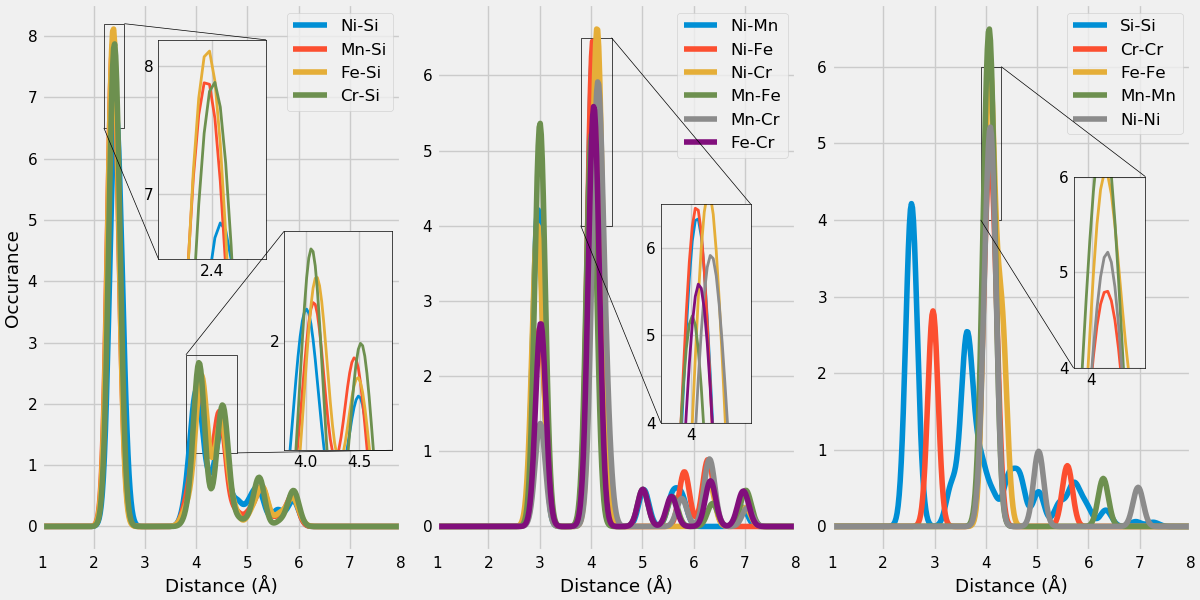
\includegraphics[width=\textwidth]{results/fesi2/D_PDF2.png}
	\end{subfigure}
	\begin{subfigure}{\textwidth}
		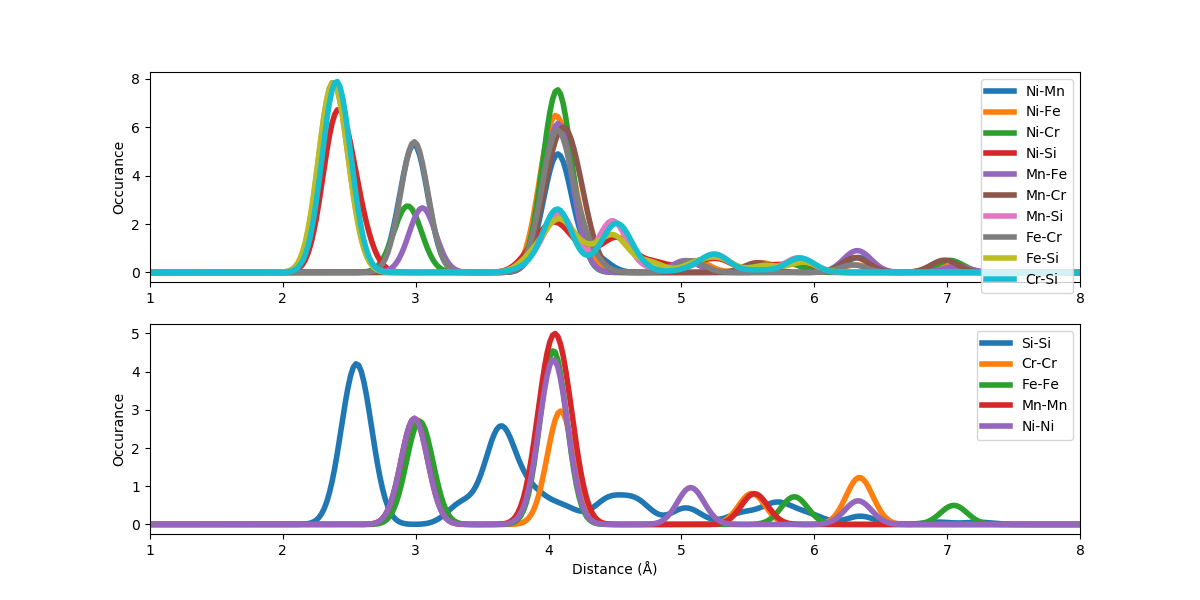
\includegraphics[width=\textwidth]{results/fesi2/B_PDF.png}
	\end{subfigure}
	\caption{Probability distribution function of SQS D (top) and B (bottom)}
\end{figure}

We see that the relative positions of the PDFs remain consistent though both SQSs. With the aid of the ICSD (insert citation), we can compare the figure .. to the expected PDFs based on a number of experiments from a host of different compounds. As our compound contain a total of 15 different bonds, comparing each one to the ICSD values would be an exhaustive process. For our purpose we are satisfied by comparing the 4 different metal-Si bonds. We find that the preferred bond-length of TM-Si is observed at two values, the most dominant being the shorter of the two. For Fe-Si these are between 2.25-2.75 and 4-5, Mn-Si 2.25-2.75 and 3.5-5. Ni-Si lie between 2.25-2.5 and 3.85-5 and Cr-Si between 2.35-2.65 and 4-5.Clearly, the PDFs of the alloys are in good agreement with the listed values for Tm-Si bonds, with the most occurring bond length falling at around 2.4 Å for all TMs, and lesser occurrence between 4.0 - 4.5 Å. The height of the respective peaks is somewhat consistent in both structures, other than slightly reduced Fe-Si occurrence at 2.4 Å in B.

In contrast to the TM-Si bonds, we observe several distinctions between metal bonds in SQS D and B. Covering all would be tedious and not to insightful, instead we emphasize the bonds of Mn and Cr as this is where we found the biggest discrepancy in the PDOS. From the different TM-TM bonds (middle) of figure 8.8 we observe that the Mn-Fe bonds are most occurring at short distances in D and bigger distances in B, meaning that manganese and iron atoms are placed further from each other in structure D. \textbf{correct?} Similarly the bonds between Cr and Fe   indicate that these atoms lie closer in B than D. In contrast the nickel and manganese/chromium bonds point to a closer distance in B for Ni-Mn and Ni-Cr in D, and a greater distance between Ni and Mn in D and Ni and Cr in B. \textbf{Litt kronglete kanskje?} In terms of the homogeneous bonds, the properties of both Cr-Cr bonds and Mn-Mn bonds are more or less alike in both structures besides some majority at shorter distance in D (The red Cr-Cr line at 3Å is underneath the grey Ni-Ni line in B in figure 8.8 (bottom right)). A more significant distinction is that both Ni-Ni and Fe-Fe bonds are found at 3 Å and 4 Å in B, but exclusively 4 Å in D.    

Both the Fe-Fe and Ni-Ni bonds are in better agreement with the ICSD histograms, as the most occurring distance for these bonds are between 4-4.9 Å and additionally around 2.5 Å. \textbf{More comparisons to ICSD, ask O.M}. As a conclusion on the PDFs of this compound, we locate a pattern where the Si-Si bonds are identical and only very minor differences between TM-Si bonds in SQS D and B. This is a result of how the structures are generated with the SQS method. In th FeSi2 structure the silicon atoms are placed as before in the new supercells, but the TM elements are "randomly" distributed. Thus, it's reasonable that also here we would find the major differences between SQSs in the PDFs.
 
Bellow we show the calculated charge density (from PBE) of structure B (left) and D (rights) \textbf{What should I say about these?}
\begin{figure}[H]
	\begin{subfigure}{.5\textwidth}
		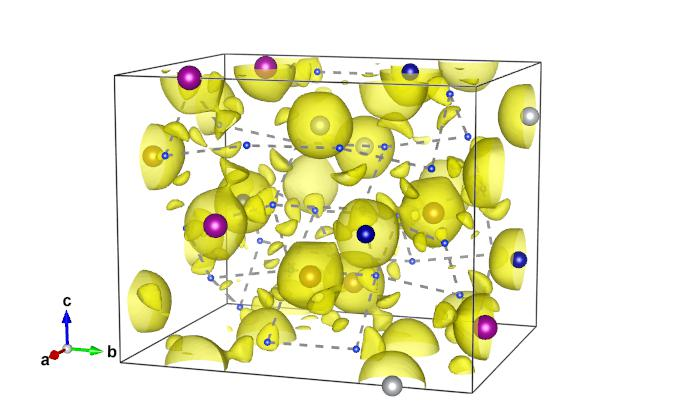
\includegraphics[width=\textwidth]{results/fesi2/B_CHGCAR.jpg}
		\caption{Structure B}
	\end{subfigure}
	\hfill
	\begin{subfigure}{.5\textwidth}
		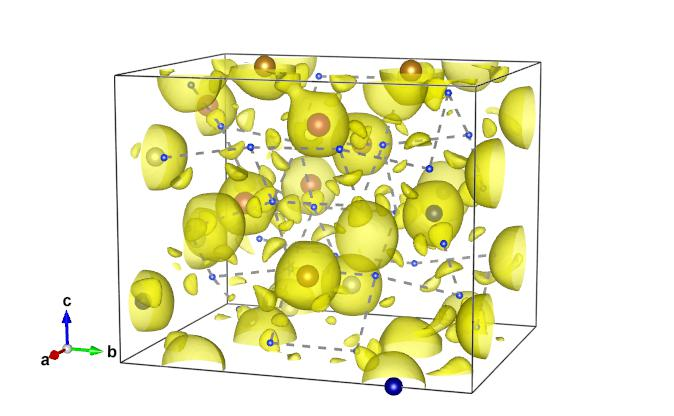
\includegraphics[width=\textwidth]{results/fesi2/D_CHGCAR.jpg}
		\caption{Structure D}
	\end{subfigure}
	\caption{Charge density of SQS D and B from PBE calculations. Illustrated by VESTA}
\end{figure}

\section{Permutations of the \ch{Cr4Fe4Mn4Ni4Si32} high-entropy silicide}
\textbf{Add Ni7, D most stable -307 eV. no band gap anywhere, not even a hint of a spin gap. Make PDOS plot and add to tables and discussion}

Up until this point we have looked in detail at the high-entropy silicide \ch{(CrFeMnNi)Si2} and associated SQSs. However these structures are just the center of a larger quasi-ternary phase diagram consisting of the different possible distributions of elements Thus there exists many more permutations of this particular composition of a high-entropy silicide. In this section, we aim to expand our search of this diagram by generating SQSs slightly away from eqvimolar distribution of 3d elements. In table (bellow) we list the mean total energy and magnetic moment per atom with standard deviation and the enthalpy of formation of 4 permutations of the \ch{(CrFeMnNi)Si2} alloy. Ideally the permutations would differ only by one element, but the TDEP implementation insist in also reducing Nickel to stay consistent with the 48 atom supercell. 

\begin{table}[h!]
%\centering
\hskip-2.5cm\begin{tabular}{@{}cccccc@{}}
\toprule
       & \multicolumn{2}{c}{Total energy/atom (eV)} & Enthalpy of formation (eV) & \multicolumn{2}{c}{Final magnetic moment ($\mu_B$)} \\ \midrule
\ch{Cr3Fe3Mn7Ni3Si32} & - 6.6947  & 0.0040 & -11.9586  & 0.1375  & 0.0186     \\
\ch{Cr5Fe5Mn3Ni3Si32} & - 6.6705  & 0.0030 & -11.1991  & 0.1127  & 0.0223     \\
\ch{Cr5Fe3Mn5Ni3Si32} & - 6.6852  & 0.0041 & -10.5200  & 0.1375  & 0.0456     \\
\ch{Cr3Fe5Mn5Ni3Si32} & - 6.6801  & 0.0036 & -12.6426  & 0.0937  & 0.0209     \\
\ch{Cr3Fe3Mn3Ni7Si32} & - 6.3921  & 0.0078 & -10.9614  & 0.0159  & 0.0101 \\ \bottomrule
\end{tabular}
\caption{Mean and stadard deviation of the total energy and magnetic moment per atom, plus enthalpy of formation of the listed mean energies (\ch{FeSi2}).}
\end{table}

The first result of table .. we make notice of is that the stability, as evaluated by the enthalpy of formation can be increased beyond the eqvimolar composition. This is accomplished in two distinct permutations, one with increments to  manganese relative to the other TM, and the other by reduction of chromium. Moreover the two respective permutations lie on the opposite side of the magnetic scale. The large magnetic moment of the manganese rich permutation and the low magnetic moment in the chromium poor permutation is very much in line with the observations made in the previous section. Recalling that in the magnetic moment in the eqvimolar composition was largely attributed to manganese and chromium atoms in the lattice. Thus increments to manganese or reduction of chromium would following impact the magnetic moment as in the two permutations. For this reason, additionally the permutation \ch{Cr5Fe3Mn5Ni3Si32} where the nonmagnetic elements is reduced and the magnetic elements are increased ,is equally magnetic. We however find no direct relation between stability and magnetism as his particular permutation is the least stable. An important property of table 8.5 is that the listed values are the mean value of the observed property for 5 distinct SQSs of the same permutation. For example we notice that while the highest magnetic moment in the first permutation is associated with the most stable SQS (from total energy considerations). The least stable supercell show the highest magnetic moment in \ch{Cr5Fe3Mn5Ni3Si32}. 

The respective band gap of the permutations (with PBE) can be seen in table ... Compared to the previous case, we find most SQSs of the permutations to exhibit a half-metallic character. 

\begin{table}[H]
\centering
\begin{tabular}{@{}ccccc@{}}
\toprule
                                                     &   & Spin up (eV) & Spin down (eV) & Total (eV) \\ \midrule
\multicolumn{1}{c|}{\multirow{5}{*}{\textbf{\ch{Cr3Fe3Mn7Ni3Si32}}}}   & A & 0.3390                & 0                       & 0                   \\
\multicolumn{1}{c|}{}                                & B & 0.4745                & 0                       & 0                   \\
\multicolumn{1}{c|}{}                                & C & 0.1342                & 0                       & 0                   \\
\multicolumn{1}{c|}{}                                & D & 0.1950                & 0.0063                  & 0.0063              \\
\multicolumn{1}{c|}{}                                & E & 0.4211                & 0                       & 0                   \\ \midrule
\multicolumn{1}{c|}{\multirow{1}{*}{\textbf{\ch{Cr5Fe5Mn3Ni3Si32}}}}   & D & 0.0674                & 0.0413                  & 0.0372              \\ \midrule
\multicolumn{1}{c|}{\multirow{5}{*}{\textbf{\ch{Cr5Fe3Mn5Ni3Si32}}}} & A & 0.2082                & 0                       & 0                   \\
\multicolumn{1}{c|}{}                                & B & 0.4053                & 0                       & 0                   \\
\multicolumn{1}{c|}{}                                & C & 0.4659                & 0                       & 0                   \\
\multicolumn{1}{c|}{}                                & D & 0.0843                & 0.0121                  & 0.0121              \\
\multicolumn{1}{c|}{}                                & E & 0.3008                & 0                       & 0                   \\ \midrule
\multicolumn{1}{c|}{\multirow{4}{*}{\textbf{\ch{Cr3Fe5Mn5Ni3Si32}}}} & A & 0.3922                & 0                       & 0                   \\
\multicolumn{1}{c|}{}                                & C & 0.1285                & 0                       & 0                   \\
\multicolumn{1}{c|}{}                                & D & 0.2595                & 0.1004                  & 1.004               \\
\multicolumn{1}{c|}{}                                & E & 0.3591                & 0.1003                  & 0.0848              \\ \midrule
\multicolumn{1}{c|}{\multirow{1}{*}{\textbf{\ch{Cr3Fe3Mn3Ni7Si32}}}} & - & -                & -                      & -                   \\ \bottomrule
\end{tabular}
\caption{Total and spin dependent band gap of 4 permutations of CFMN (fesi2) with PBE GGA calculation. The structures that are excluded from this list either failed in calculations, or does not show any band gap.<}
\end{table}

From table ..  we see that likewise to the stability and magnetization also the band gap changes in the different directions. To some degree we find positive results of the band gap in each direction, but we see particularly that permutations rich in manganese provide very encouraging results. This is made clear from the fact that \ch{Cr3Fe3Mn7Ni3Si32}, \ch{Cr5Fe3Mn5Ni3Si32} and \ch{Cr3Fe5Mn5Ni3Si32} all include amounts of manganese higher than the eqvimolar composistion and all associated SQSs show at least strong half-metalic charachter or semiconducting. On the other side \ch{Cr5Fe5Mn3Ni3Si32} is the sole permutation with less manganse and correspondingly show the least sign of a band gap. Moreover the relative stability of the SQSs give further merit to the proposition. In the first permutation we find that the highest total energy is associated with SQS B, which as seen in table .. exhibit the largest spin up band gap of the particular permutation. Furthermore the two semiconducting SQSs in the last permutation is the two most stable arrangements. Reversely, in the manganese-poor permutation we find that the sole semiconducting SQS is the second least stable of that compound. Lastly, the opposite is the case is true in the third permutation. Despite the total energy not varying tremendously between SQSs of the same permutation, as seen by the standard deviation in table .., the continuing trend between stability and band gap is a promising result to report.

In figure 8.12 we plot the projected density of states around $E_F$ of the 4 permutations. Note that away from the Fermi energy the projected density of states is analogous to the parent compound, see appendix ..

\begin{figure}[H]
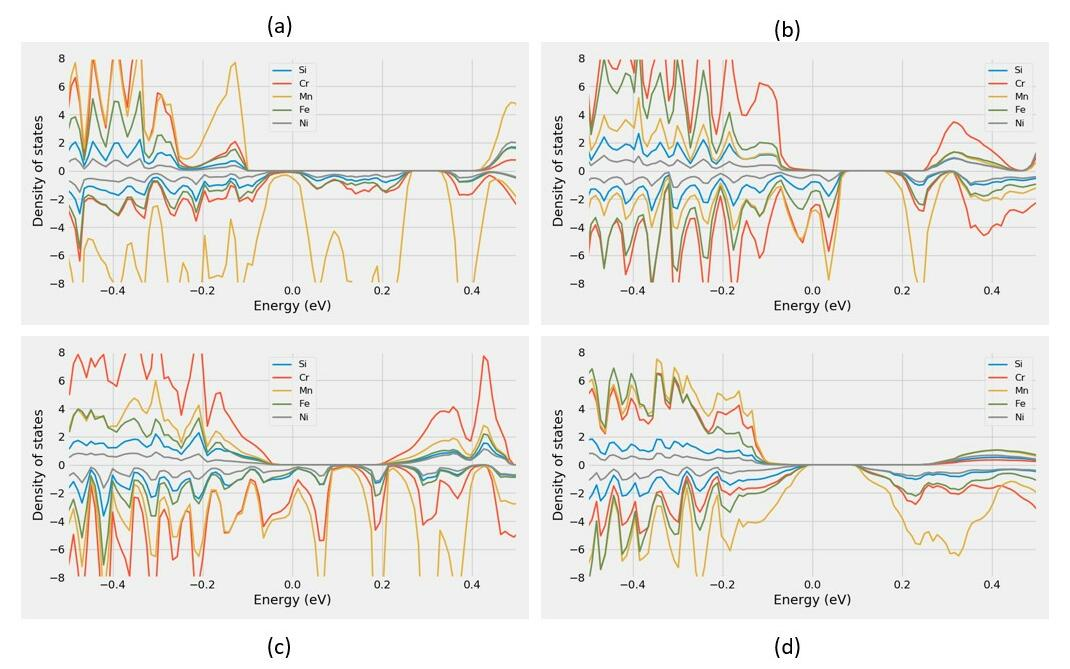
\includegraphics[width=\linewidth]{results/fesi2/permutations/perm_LDOS_crop.jpg}
\caption{Projected density of states of (a) \ch{Cr3Fe3Mn7Ni3Si32} (SQS B), (b) \ch{Cr5Fe5Mn3Ni3Si32} (SQS C), (c) \ch{Cr5Fe3Mn5Ni3Si32} (SQS A), (d) \ch{Cr3Fe5Mn5Ni3Si32} (SQS D)}
\end{figure}

The above figures is based on the most stable SQS in each permutation, as will the analysis. Thus the features of these figures does not necessarily represent the complete set of SQSs of the permutation. As experienced in table 8.6 and previous examples in this project, the band gap and properties of each permutation can vary between SQSs. But given that the structures came out on top in terms of total energy means that they are the most probable configuration of the real alloy, hence also the features of that supercell. 

With that said, the plotted PDOSs in figure 8.12 clearly illustrate the characteristics shown in table 8.6. We see clear indication of a spin up band gap in \ch{Cr3Fe3Mn7Ni3Si32} (a) and \ch{Cr5Fe3Mn5Ni3Si32} (c), and a total band gap in \ch{Cr3Fe5Mn5Ni3Si32} (d). Not so clear is that the density of states of \ch{Cr5Fe5Mn3Ni3Si32} (b) contain very small nonzero values at $E_F$ and the unoccupied states is shifted very slightly above the Fermi energy, prohibiting an otherwise clear band gap. In figure 8.13 the total density of states of SQS D and E of this permutation is shown, the above point is seen also in SQS E, where the "band gap" is shifted above $E_F$.
 
\begin{figure}[H]
	\begin{subfigure}{.5\textwidth}
		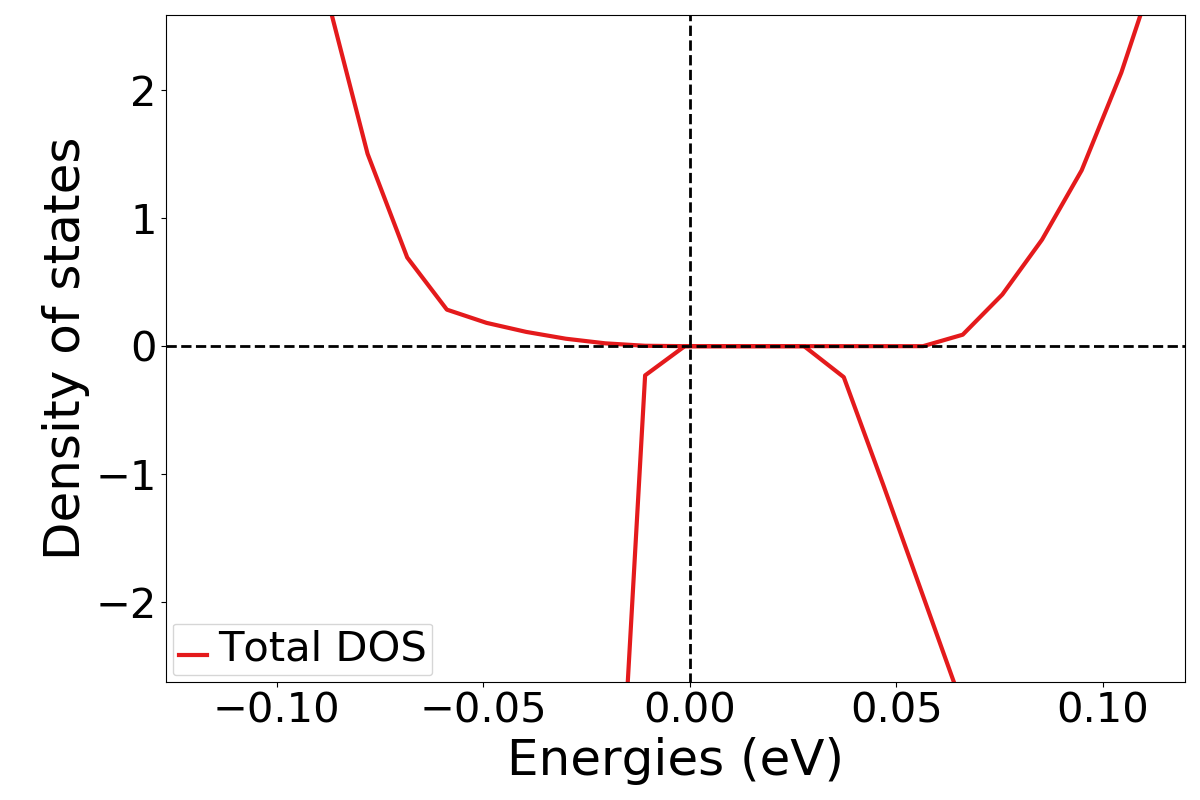
\includegraphics[width=\textwidth]{results/fesi2/permutations/mnni3_DOS.png}
		\caption{SQS D}
	\end{subfigure}
	\begin{subfigure}{.5\textwidth}
		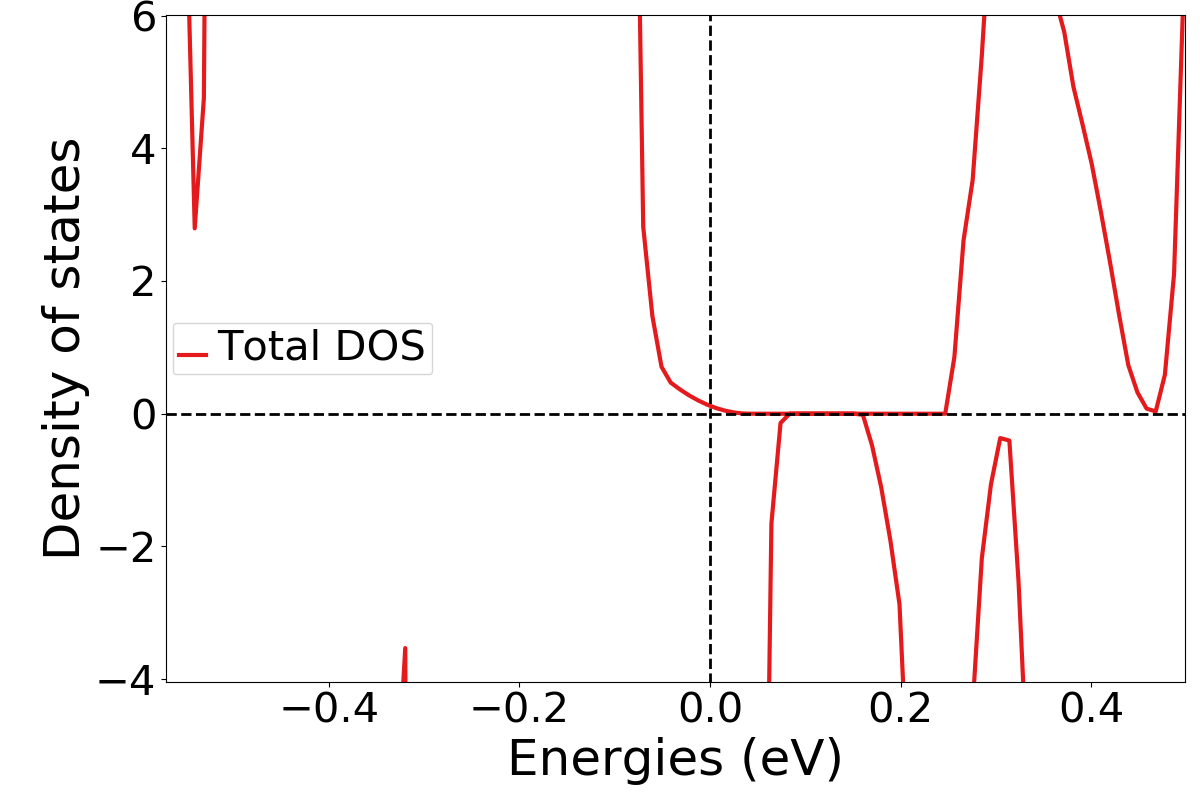
\includegraphics[width=\textwidth]{results/fesi2/permutations/mnni3_DOS_E.png}
		\caption{SQS E}
	\end{subfigure}
	\caption{Density of states around $E_F$ of SQS D and E \ch{Cr5Fe5Mn3Ni3Si32}}
\end{figure}


In figure 8.6 we saw that electrons from manganese atoms in particular was a key contributor as to why the spin down channel of \ch{(CrFeMnNi)Si2} was metallic in the stable supercell D. This is also largely the case in the permutations shown above in figure 8.12.    
 
The proportion of manganese atoms in the alloy seems to offer a very positive effect on the band gap in spin up, but is often detrimental to spin down. This is seen in figure 8.12 (a) and (c) for \ch{Cr3Fe3Mn7Ni3Si32} and \ch{Cr5Fe3Mn5Ni3Si32} respectively, that both contain increased amounts of manganese. By reducing the number of Mn as in (b) we still find that the Mn electrons plague the states at $E_F$ in spin down. In analog we see from (b) and (c) that also Cr negatively impacts to the band gap especially in spin up. The sole permutation with clear evidence of a spin down gap is from the chromium poor permutation plotted in (d). Also in this structure we see that the effects of Mn around $E_F$ is dampened in comparison to the other permutations, despite containing relatively increased amounts of Mn to the eqvimolar alloy.  

\begin{figure}[H]
	\centering
	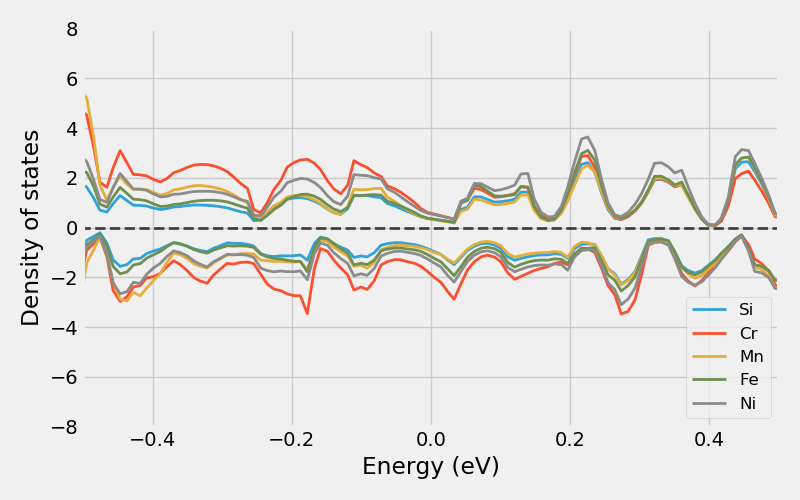
\includegraphics[width=.6\textwidth]{results/fesi2/permutations/ni7_PDOS.png}
	\caption{Projected density of states of \ch{Cr3Fe3Mn3Ni7Si32} around $E_F$}
\end{figure}

An important property of these results is that because each permutation alters simultaneous elements, interpreting and relating the results to a particular alteration is challenging. For example, is the result of the \ch{Cr5Fe3Mn5Ni3Si32} permutation a consequence of less Fe or increments to both Cr and Mn? Furthermore is the exaggerated band gap in spin up of \ch{Cr3Fe3Mn7Ni3Si32} a product of increasing manganese or reducing the other elements. From the comparatively large gaps in spin up of \ch{Cr3Fe3Mn7Ni3Si32} and \ch{Cr3Fe5Mn5Ni3Si32} and the more present Cr states in spin up in the Cr rich permutations we here conclude that the band gap is related to lessening of chromium, more so than other effects. Despite of this we generally find positive results regarding most of the permutations as seen in table 8.6, the exception to this \ch{Cr3Fe3Mn3Ni3si32}. This particular permutation in opposition to the others in this section increases the proportion of Ni at the cost of the other 3d elements. The projected density of states is displayed in figure [REF]. From both this structure, but also the PDOS of \ch{Cr3Fe3Mn7Ni3Si32} we see that reducing chromium does not always improve the band gap. It's clear that the \ch{Cr3Fe5Mn5Ni3Si32} alloy manage to strike a balance of distribution that results in a specific interplay between the 3d elements. For this reason we more closely investigate the properties of this structure.

\begin{figure}[H]
	\centering
	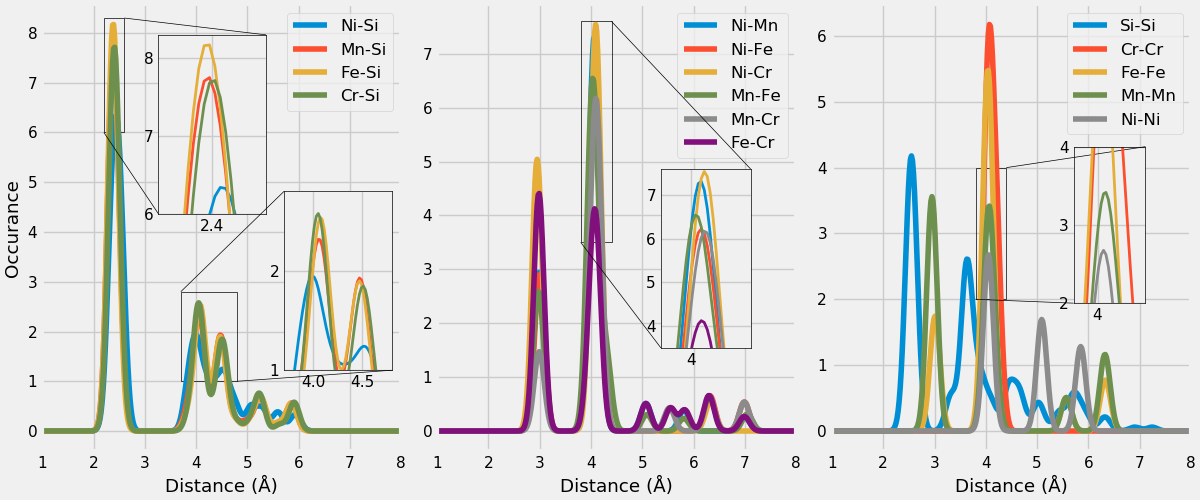
\includegraphics[width=\textwidth]{results/fesi2/permutations/_crni3_D_PDF.png}
	\caption{Probability distribution functions to \ch{Cr3Fe5Mn5Ni3Si32} SQS D, \textbf{Maybe make larger}}
\end{figure}

\textbf{Comment figure \\}

\textbf{Add some figures from HSE06?}
In this segment of the project we scarcely applied the more advanced functionals SCAN and HSE06, in part to both the uncertainties mentioned in the previous section and the computational cost of the methods. However we did perform such calculations (HSE06) to further investigate the nature of the listed semiconducting SQSs. Both the manganese rich and poor semiconductors are validated with the HSE06 functional and find wider band gaps of 0.17 eV (0.57 and 0.26 in up and down) in \ch{Cr3Fe3Mn7Ni3Si32} SQS D, and 0.22 eV (0.77 eV in spin up) in \ch{Cr5Fe5Mn3Ni3Si32} SQS D. On the opposite side, the very narrow band gap in \ch{Cr5Fe3Mn5Ni3Si32} vanishes with HSE06 calculations. For the two stable semiconductors found in \ch{Cr3Fe5Mn5Ni3Si32}, simulations with the HSE06 functional resulted in a half-metal with a spin up of 0.53 eV for SQS D, and a total band-gap of 0.27 eV for E, where the spin-up gap is 0.73 eV wide.

\textbf{Conclusion this section}
